\chapter{}

\section{ADNI extra figures}
\label{sec:adni_extra_appendix}

% \tikzset{every picture/.append style={scale=0.6}}

\newcommand*{\midLateralLoc}{../drawImages/input/images}
% scale parameter for the font size in the circles
\newcommand*{\scaleLabelImg}{0.7}
\begin{figure}[h]
  \centering
  \includegraphics*[scale=\scaleLabelImg]{\midLateralLoc/Mid-Lateral_surface3.eps}
  \caption{Labels of the different areas analysed in the EBM progression snapshots from chapter \ref{chapter:ebm}. }
  \label{fig:ebmSnapLabels}
\end{figure}

\vspace{10cm}

\section{Performance evaluation - Synthetic results}

\newcommand{\ctlPrecCaption}{ \caption{increasing precision of the control group diagnosis, i.e. the controls start from being spread along the disease course to being only at the very early stages. }}

\newcommand{\simFigScale}{0.45}


\begin{figure}[H]
%\centering
 \hspace{-2cm}
 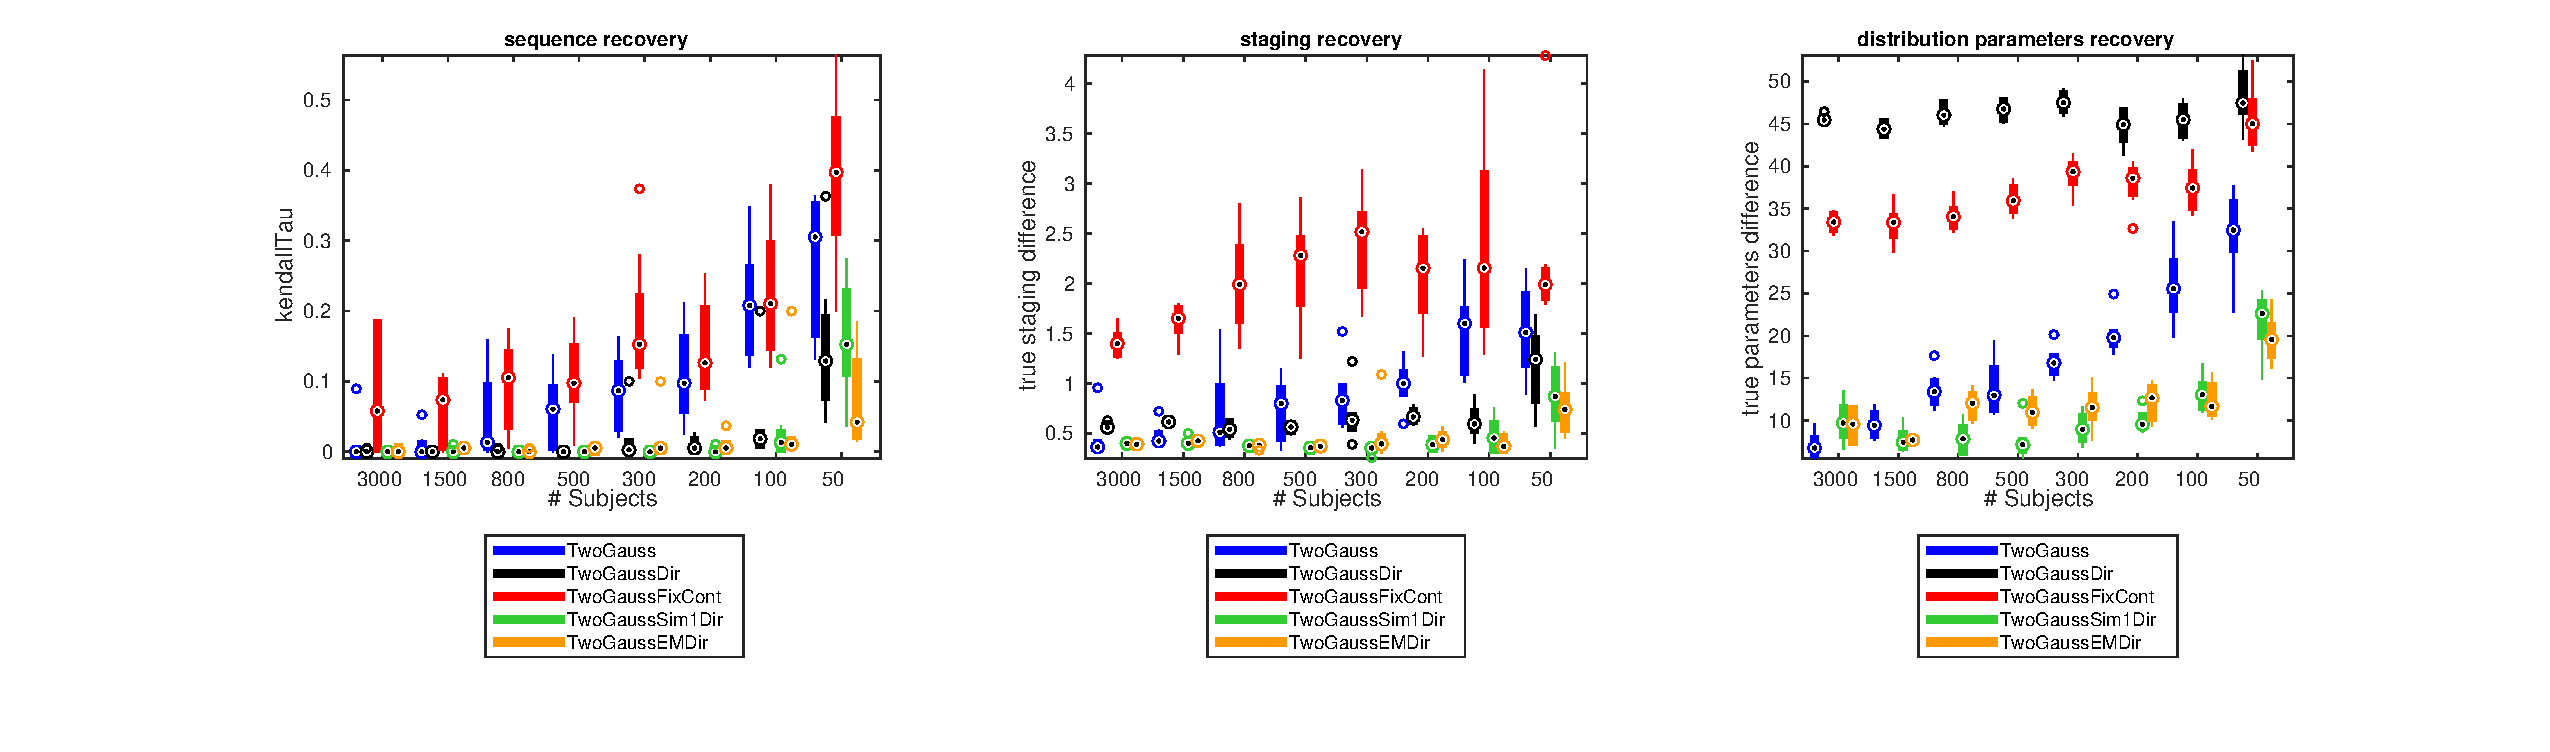
\includegraphics[scale=\simFigScale]{images/ebm/synthetic/metricsTwoGauss_incrSubj.eps}
\caption{Simulation results comparing different EBM model fitting methods. In blue we have the standard EBM method which first fits the distribution parameters and then the sequence, while in black and red we have the EBM Expectation-Maximisation method with two different starting points. Each of these three methods have been fit on eight synthetic datasets where we used a decreasing number of subjects, from 3000 down to 50. The left figure shows the Kendall-tau distance between the sequence recovered by the model and the true sequence. The middle figure shows the L1 norm of the difference between predicted subject stages and true stages. The right figure shows the L1 norm of the difference between the recovered distribution parameters and the true parameters.}
 \label{fig:incrSubjTG}
\end{figure}

\begin{table}[H]
\centering
\begin{tabular}{c | p{13cm}}
 TwoGauss & fit distribution parameters by optimising a mixture model, like Fontejin et al. \cite{fonteijn2012event}, Young et al. \cite{young2014data}\\
 TwoGaussDir & fitting each distribution directly on the control and patient data, optimise sequence independenly\\
 TwoGaussFixCont & fit the control distribution directly on control data, then fit patient distribution using mixture model optimisation.\\
 TwoGaussSim1 & simultaneous sampling of parameters and sequence, initialise the method from the solution found by TwoGauss\\
 TwoGaussSim1Dir & same as TwoGaussSim1, initialise the method from the solution found by TwoGaussDir\\
 
\end{tabular}
\caption{Legend description for Fig. \ref{fig:incrSubjTG}}
\end{table}

\begin{figure}[H]
%\centering
 \hspace{-2cm}
 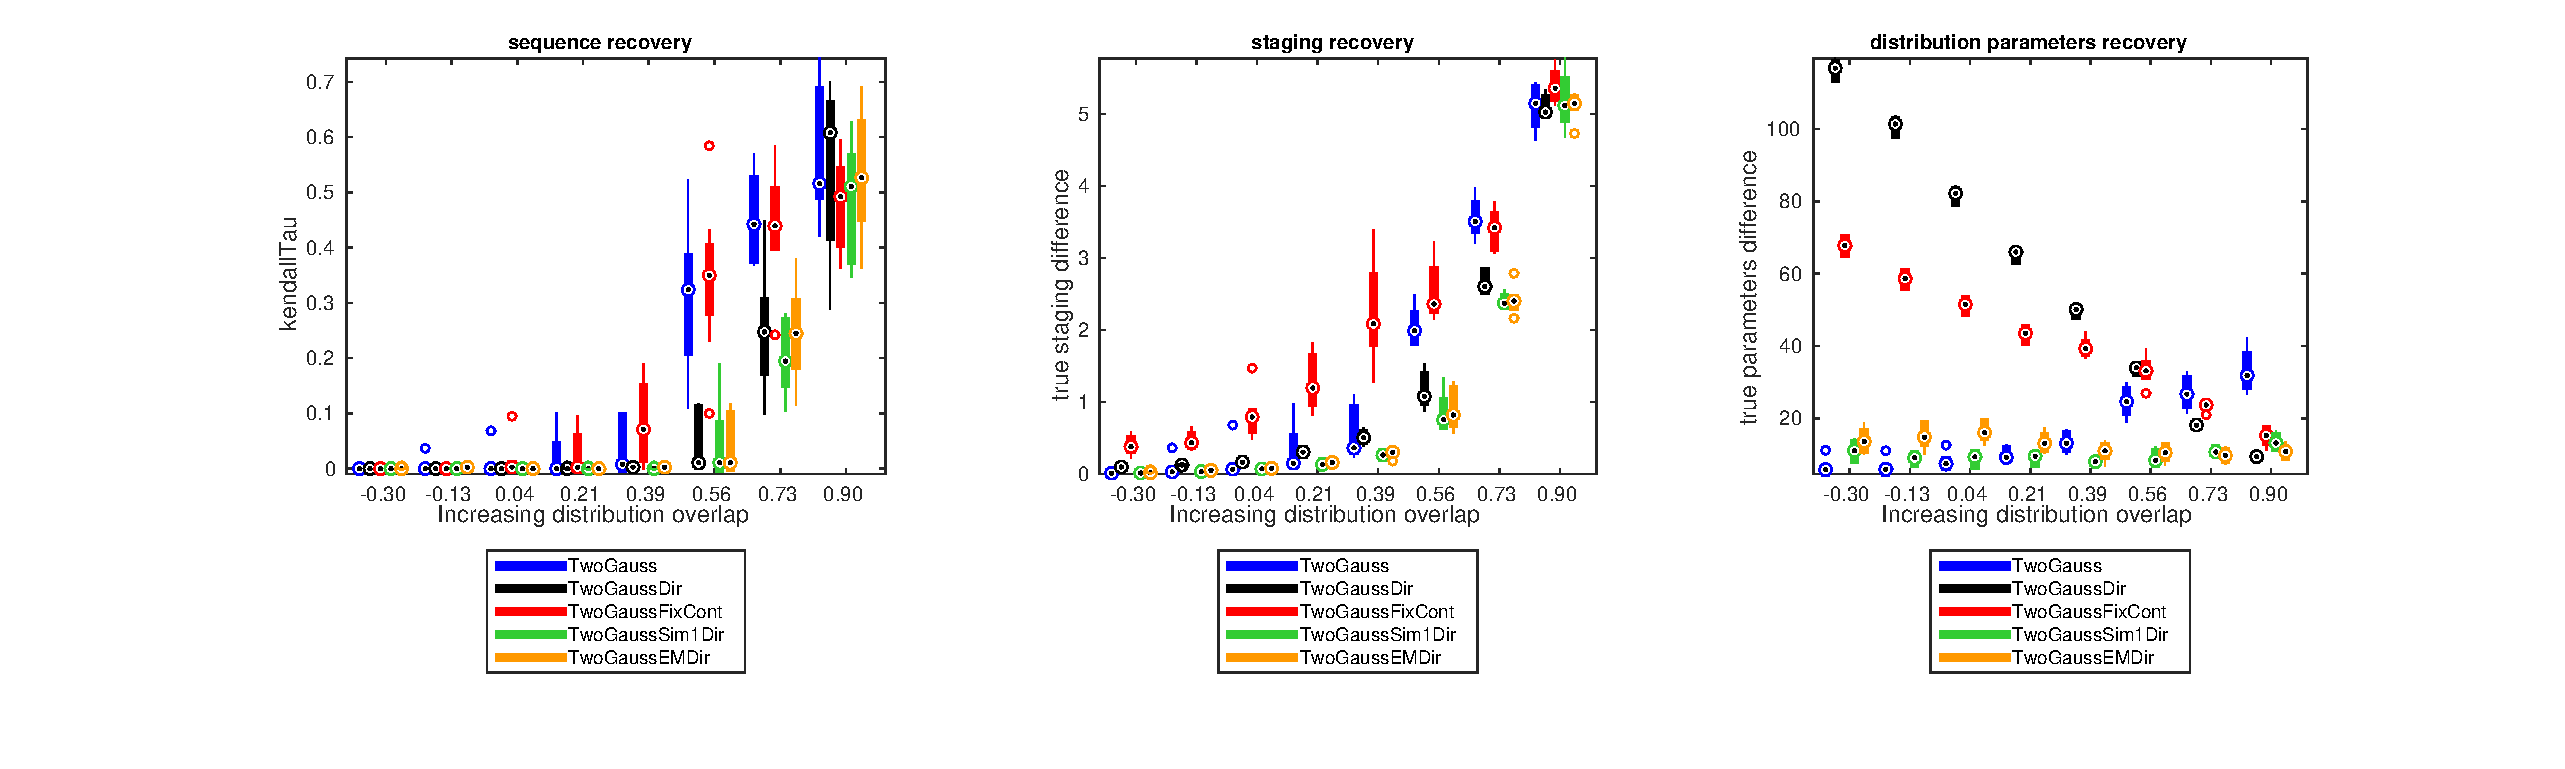
\includegraphics[scale=\simFigScale]{images/ebm/synthetic/metricsTwoGauss_incrDistOverlap.eps}
 \caption{Simulation results comparing different EBM model fitting methods. Same setup as in Fig. \ref{fig:incrSubjTG}, but this time we keep the number of subjects constant and instead increase the overlap of distributions $p(x|E)$ and $p(x| \neg E)$. The distribution overlap ranges from -0.3 (low overlap) to 0.9 (high overlap). } 
  \label{fig:incrDstTG}
\end{figure}

\begin{figure}[H]
%\centering
 \hspace{-2cm}
 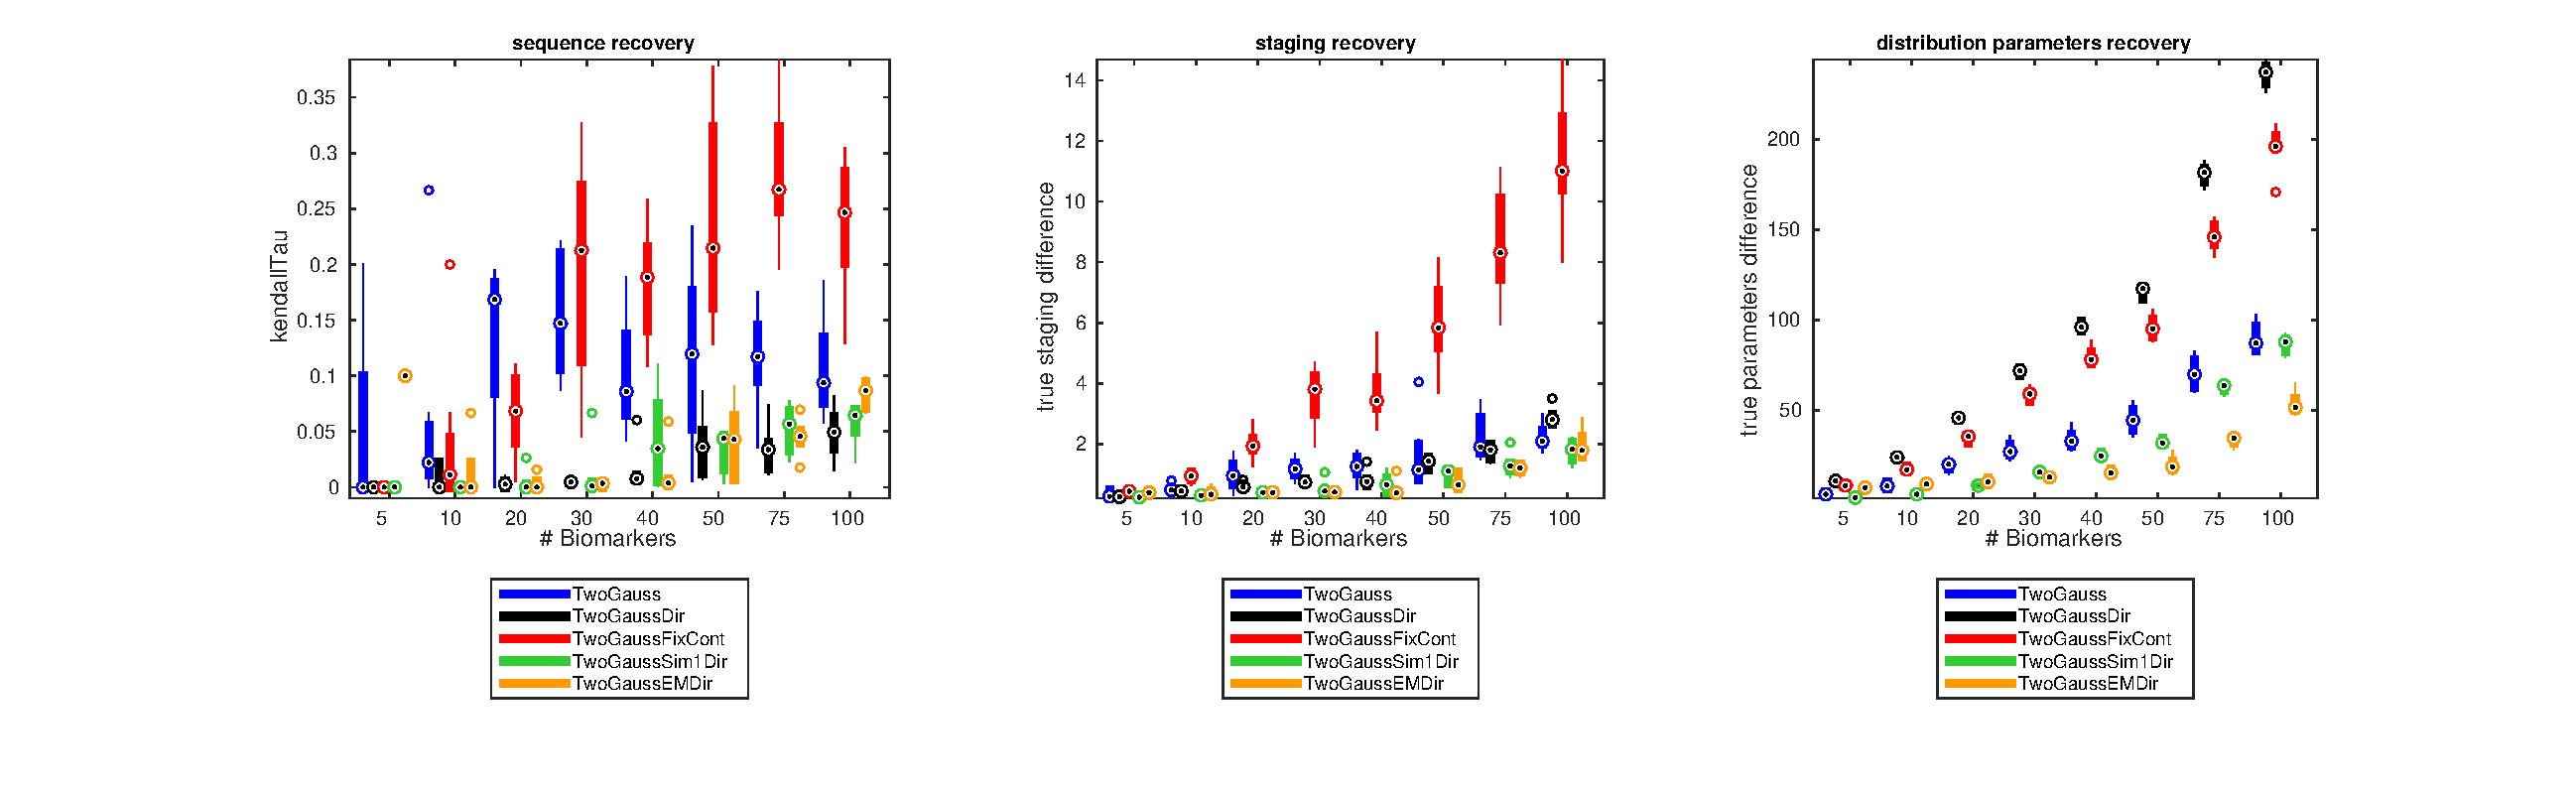
\includegraphics[scale=\simFigScale]{images/ebm/synthetic/metricsTwoGauss_incrBiomk.eps}
\caption{Simulation results comparing different EBM model fitting methods. Same setup as in Fig. \ref{fig:incrSubjTG}, but this time we keep the number of biomarkers used, from 0 to 100.}
  \label{fig:incBiomkTG}
\end{figure}

\begin{figure}[H]
%\centering
 \hspace{-2cm}
 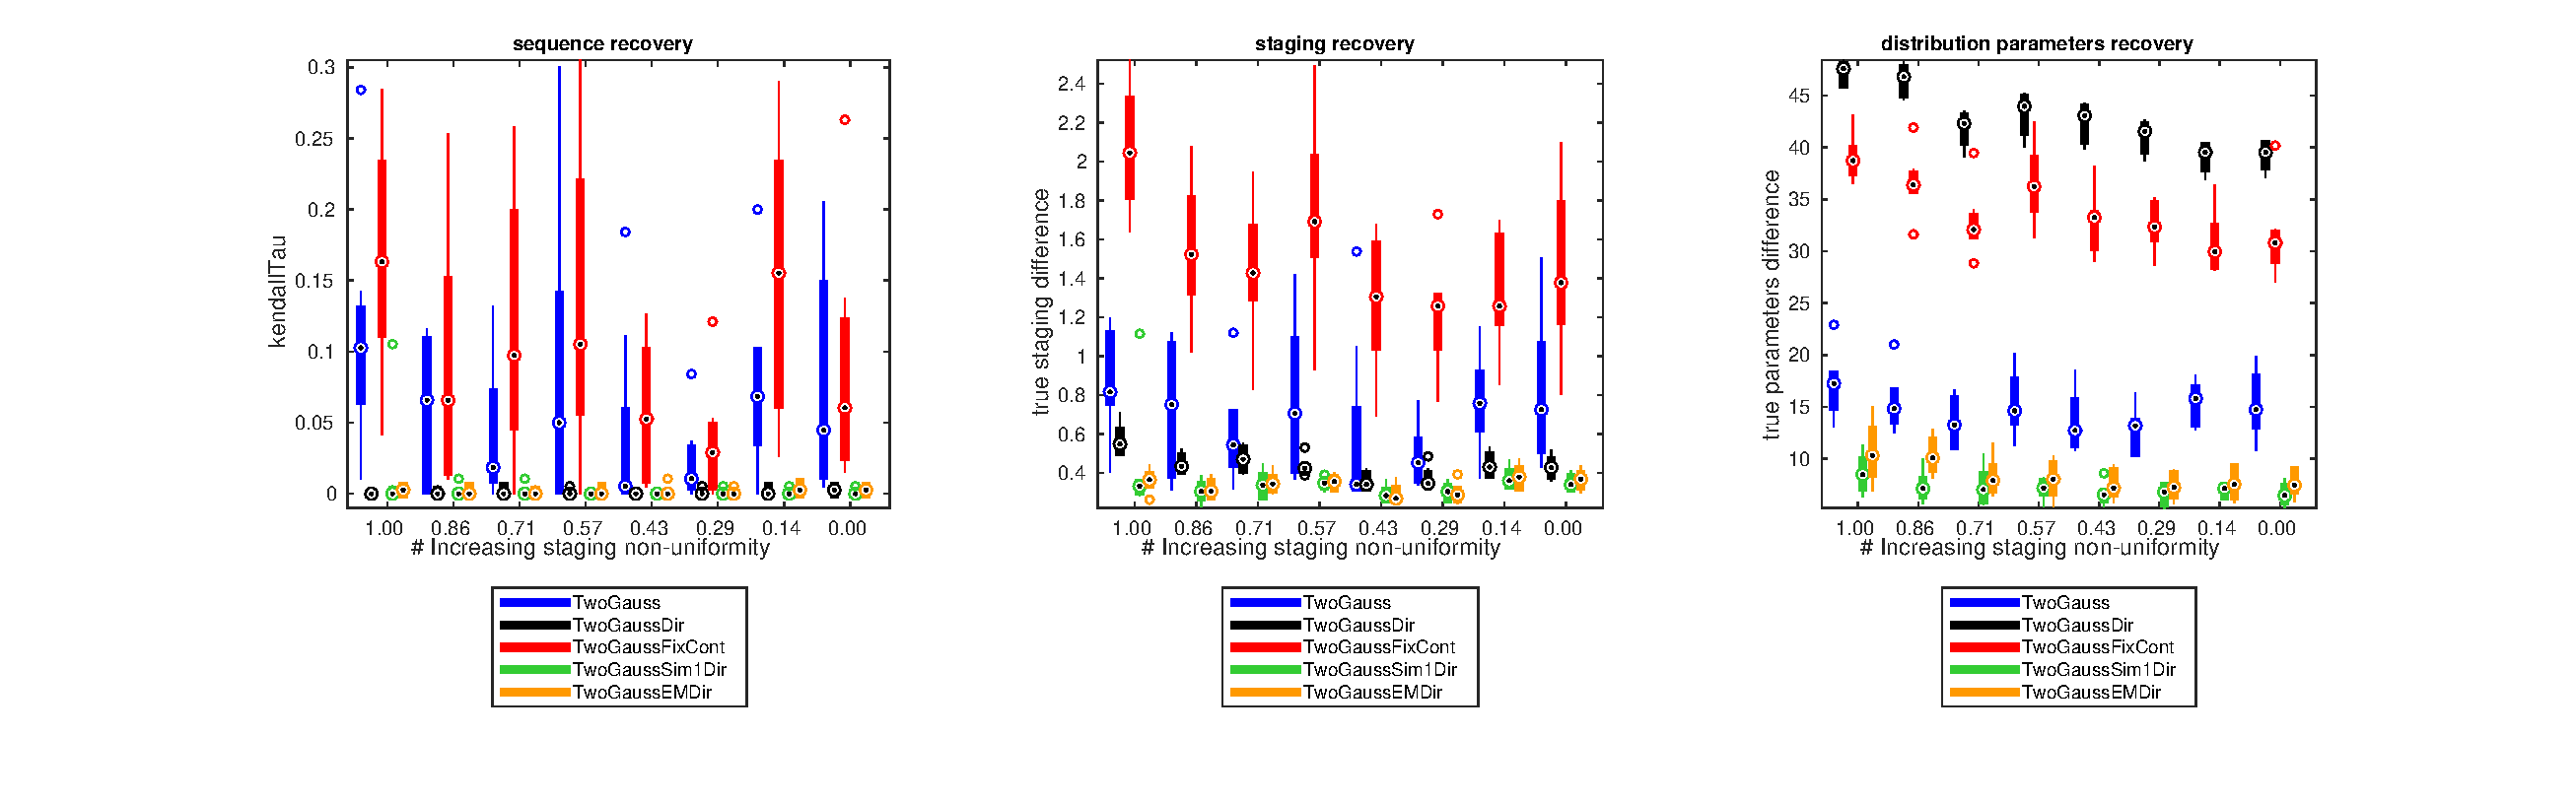
\includegraphics[scale=\simFigScale]{images/ebm/synthetic/metricsTwoGauss_incrStagingUnif.eps}
 \caption{Simulation results comparing different EBM model fitting methods. Same setup as in Fig. \ref{fig:incrSubjTG}, but this time we vary the uniformity of the subject stages, ranging from 1 (uniform probability across the disease timecourse) to 0 (subjects are placed more at beginning or end stages). The pdfs of the stage distributions for each experiment are shown in Fig. \ref{fig:StagingCurvesTG}. }
  \label{fig:incrStagTG}
\end{figure}

\begin{figure}[H]
 \centering
 \hspace{-2cm}
 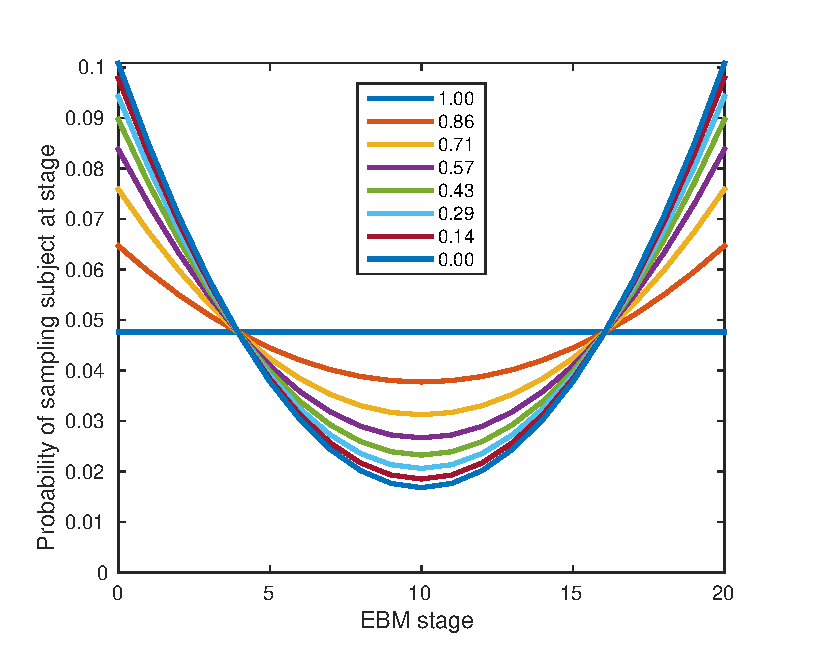
\includegraphics[scale=\simFigScale]{images/ebm/synthetic/stagingUnifCurves.eps}
 \caption{Pdf of the staging probability functions used to generate the synthetic datasets in Fig. \ref{fig:incrStagTG}. The shapes of the pdf distributions are quadratic curves for which we vary the second-order factor.}
 \label{fig:StagingCurvesTG}
\end{figure}

\begin{figure}[H]
%\centering
 \hspace{-2cm}
 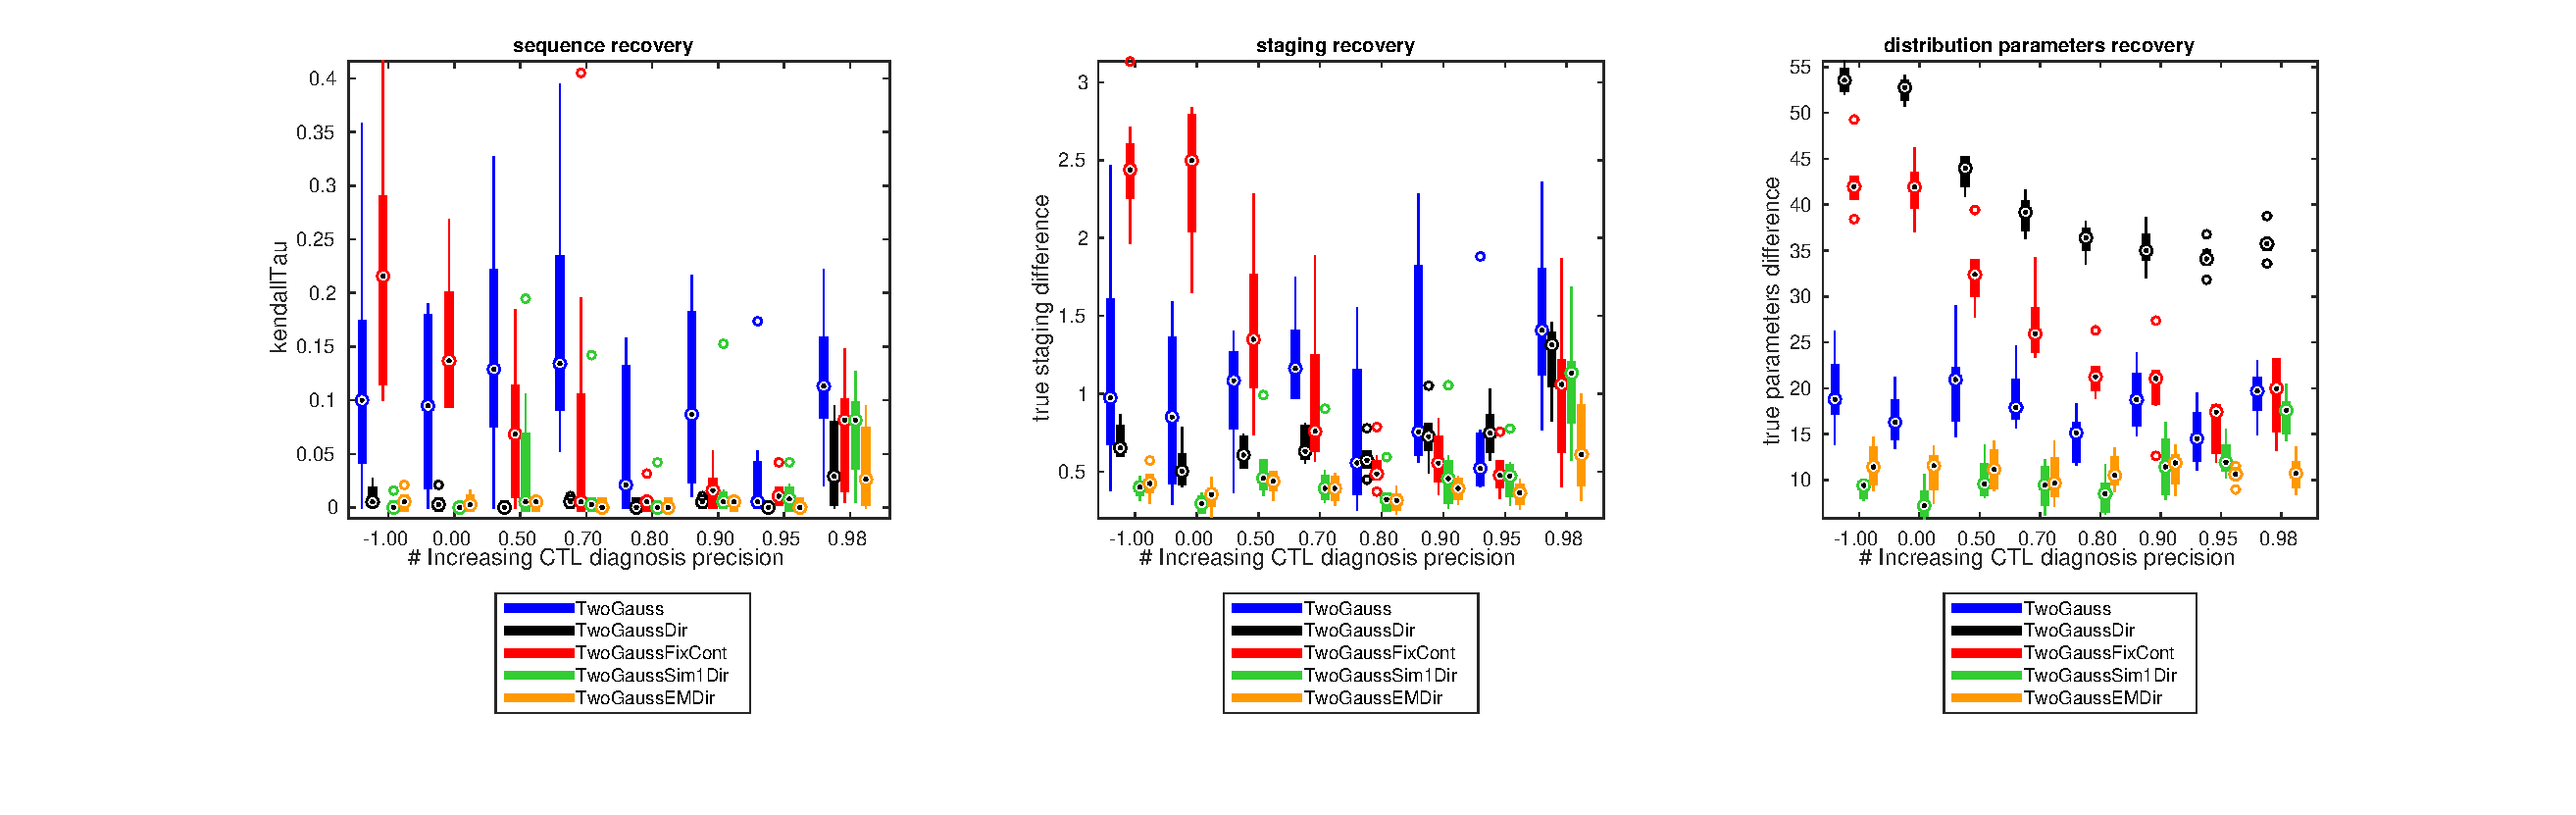
\includegraphics[scale=\simFigScale]{images/ebm/synthetic/metricsTwoGauss_incrCtlPrec.eps}
 \caption{Simulation results comparing different EBM model fitting methods. Same setup as in Fig. \ref{fig:incrSubjTG}, but this time we vary the precision of the control distribution, ranging from -1 (well-defined control population) to 1 (not so well defined control population). The pdfs of the stage distribution for control subjects in each experiment are shown in Fig. \ref{fig:ctlPrecCurvesTG}. }
  \label{fig:incrCtlPrecTG}
\end{figure}

\begin{figure}[H]
 \centering
 \hspace{-2cm}
 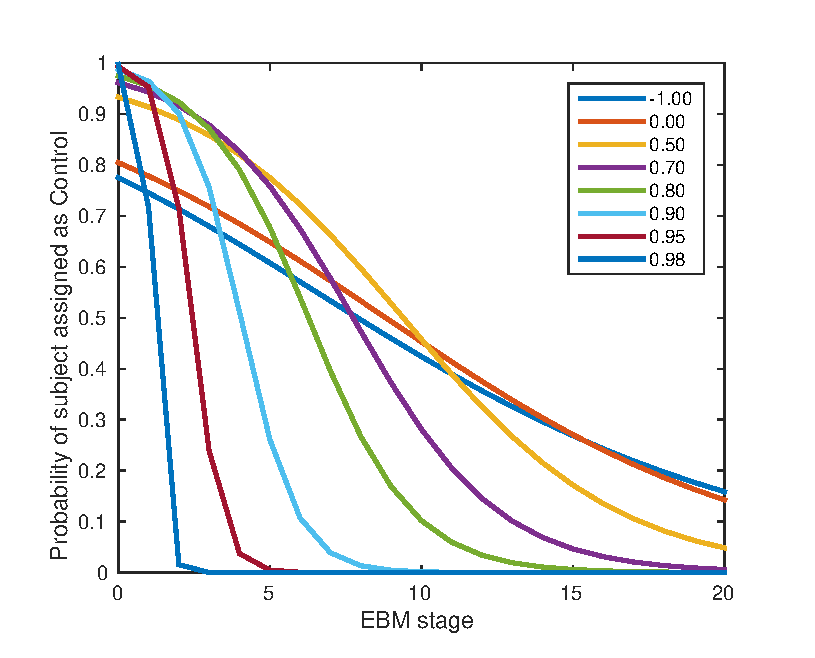
\includegraphics[scale=\simFigScale]{images/ebm/synthetic/ctlPrecCurves.eps}
 \caption{Probability density functions for the sampling distribution of the stages of controls. This ranges from -1 (well-defined control population) to 1 (not so well defined control population)}
 \label{fig:ctlPrecCurvesTG}
\end{figure}